
%% bare_conf.tex
%% V1.4b
%% 2015/08/26
%% by Michael Shell
%% See:
%% http://www.michaelshell.org/
%% for current contact information.
%%
%% This is a skeleton file demonstrating the use of IEEEtran.cls
%% (requires IEEEtran.cls version 1.8b or later) with an IEEE
%% conference paper.
%%
%% Support sites:
%% http://www.michaelshell.org/tex/ieeetran/
%% http://www.ctan.org/pkg/ieeetran
%% and
%% http://www.ieee.org/

%%*************************************************************************
%% Legal Notice:
%% This code is offered as-is without any warranty either expressed or
%% implied; without even the implied warranty of MERCHANTABILITY or
%% FITNESS FOR A PARTICULAR PURPOSE!
%% User assumes all risk.
%% In no event shall the IEEE or any contributor to this code be liable for
%% any damages or losses, including, but not limited to, incidental,
%% consequential, or any other damages, resulting from the use or misuse
%% of any information contained here.
%%
%% All comments are the opinions of their respective authors and are not
%% necessarily endorsed by the IEEE.
%%
%% This work is distributed under the LaTeX Project Public License (LPPL)
%% ( http://www.latex-project.org/ ) version 1.3, and may be freely used,
%% distributed and modified. A copy of the LPPL, version 1.3, is included
%% in the base LaTeX documentation of all distributions of LaTeX released
%% 2003/12/01 or later.
%% Retain all contribution notices and credits.
%% ** Modified files should be clearly indicated as such, including  **
%% ** renaming them and changing author support contact information. **
%%*************************************************************************


% *** Authors should verify (and, if needed, correct) their LaTeX system  ***
% *** with the testflow diagnostic prior to trusting their LaTeX platform ***
% *** with production work. The IEEE's font choices and paper sizes can   ***
% *** trigger bugs that do not appear when using other class files.       ***
% The testflow support page is at:
% http://www.michaelshell.org/tex/testflow/



\documentclass[conference]{IEEEtran}
% Some Computer Society conferences also require the compsoc mode option,
% but others use the standard conference format.
%
% If IEEEtran.cls has not been installed into the LaTeX system files,
% manually specify the path to it like:
% \documentclass[conference]{../sty/IEEEtran}





% Some very useful LaTeX packages include:
% (uncomment the ones you want to load)


% *** MISC UTILITY PACKAGES ***
%
%\usepackage{ifpdf}
% Heiko Oberdiek's ifpdf.sty is very useful if you need conditional
% compilation based on whether the output is pdf or dvi.
% usage:
% \ifpdf
%   % pdf code
% \else
%   % dvi code
% \fi
% The latest version of ifpdf.sty can be obtained from:
% http://www.ctan.org/pkg/ifpdf
% Also, note that IEEEtran.cls V1.7 and later provides a builtin
% \ifCLASSINFOpdf conditional that works the same way.
% When switching from latex to pdflatex and vice-versa, the compiler may
% have to be run twice to clear warning/error messages.






% *** CITATION PACKAGES ***
%
\usepackage{cite}
% cite.sty was written by Donald Arseneau
% V1.6 and later of IEEEtran pre-defines the format of the cite.sty package
% \cite{} output to follow that of the IEEE. Loading the cite package will
% result in citation numbers being automatically sorted and properly
% "compressed/ranged". e.g., [1], [9], [2], [7], [5], [6] without using
% cite.sty will become [1], [2], [5]--[7], [9] using cite.sty. cite.sty's
% \cite will automatically add leading space, if needed. Use cite.sty's
% noadjust option (cite.sty V3.8 and later) if you want to turn this off
% such as if a citation ever needs to be enclosed in parenthesis.
% cite.sty is already installed on most LaTeX systems. Be sure and use
% version 5.0 (2009-03-20) and later if using hyperref.sty.
% The latest version can be obtained at:
% http://www.ctan.org/pkg/cite
% The documentation is contained in the cite.sty file itself.






% *** GRAPHICS RELATED PACKAGES ***
%
\ifCLASSINFOpdf
    \usepackage[pdftex]{graphicx}
  % declare the path(s) where your graphic files are
  % \graphicspath{{../pdf/}{../jpeg/}}
  % and their extensions so you won't have to specify these with
  % every instance of \includegraphics
  % \DeclareGraphicsExtensions{.pdf,.jpeg,.png}
\else
  % or other class option (dvipsone, dvipdf, if not using dvips). graphicx
  % will default to the driver specified in the system graphics.cfg if no
  % driver is specified.
  % \usepackage[dvips]{graphicx}
  % declare the path(s) where your graphic files are
  % \graphicspath{{../eps/}}
  % and their extensions so you won't have to specify these with
  % every instance of \includegraphics
  % \DeclareGraphicsExtensions{.eps}
\fi
% graphicx was written by David Carlisle and Sebastian Rahtz. It is
% required if you want graphics, photos, etc. graphicx.sty is already
% installed on most LaTeX systems. The latest version and documentation
% can be obtained at:
% http://www.ctan.org/pkg/graphicx
% Another good source of documentation is "Using Imported Graphics in
% LaTeX2e" by Keith Reckdahl which can be found at:
% http://www.ctan.org/pkg/epslatex
%
% latex, and pdflatex in dvi mode, support graphics in encapsulated
% postscript (.eps) format. pdflatex in pdf mode supports graphics
% in .pdf, .jpeg, .png and .mps (metapost) formats. Users should ensure
% that all non-photo figures use a vector format (.eps, .pdf, .mps) and
% not a bitmapped formats (.jpeg, .png). The IEEE frowns on bitmapped formats
% which can result in "jaggedy"/blurry rendering of lines and letters as
% well as large increases in file sizes.
%
% You can find documentation about the pdfTeX application at:
% http://www.tug.org/applications/pdftex





% *** MATH PACKAGES ***
%
\usepackage{amsmath}
% A popular package from the American Mathematical Society that provides
% many useful and powerful commands for dealing with mathematics.
%
% Note that the amsmath package sets \interdisplaylinepenalty to 10000
% thus preventing page breaks from occurring within multiline equations. Use:
%\interdisplaylinepenalty=2500
% after loading amsmath to restore such page breaks as IEEEtran.cls normally
% does. amsmath.sty is already installed on most LaTeX systems. The latest
% version and documentation can be obtained at:
% http://www.ctan.org/pkg/amsmath





% *** SPECIALIZED LIST PACKAGES ***
%
%\usepackage{algorithmic}
% algorithmic.sty was written by Peter Williams and Rogerio Brito.
% This package provides an algorithmic environment fo describing algorithms.
% You can use the algorithmic environment in-text or within a figure
% environment to provide for a floating algorithm. Do NOT use the algorithm
% floating environment provided by algorithm.sty (by the same authors) or
% algorithm2e.sty (by Christophe Fiorio) as the IEEE does not use dedicated
% algorithm float types and packages that provide these will not provide
% correct IEEE style captions. The latest version and documentation of
% algorithmic.sty can be obtained at:
% http://www.ctan.org/pkg/algorithms
% Also of interest may be the (relatively newer and more customizable)
% algorithmicx.sty package by Szasz Janos:
% http://www.ctan.org/pkg/algorithmicx




% *** ALIGNMENT PACKAGES ***
%
\usepackage{array}
% Frank Mittelbach's and David Carlisle's array.sty patches and improves
% the standard LaTeX2e array and tabular environments to provide better
% appearance and additional user controls. As the default LaTeX2e table
% generation code is lacking to the point of almost being broken with
% respect to the quality of the end results, all users are strongly
% advised to use an enhanced (at the very least that provided by array.sty)
% set of table tools. array.sty is already installed on most systems. The
% latest version and documentation can be obtained at:
% http://www.ctan.org/pkg/array


% IEEEtran contains the IEEEeqnarray family of commands that can be used to
% generate multiline equations as well as matrices, tables, etc., of high
% quality.




% *** SUBFIGURE PACKAGES ***
\ifCLASSOPTIONcompsoc
  \usepackage[caption=false,font=normalsize,labelfont=sf,textfont=sf]{subfig}
\else
  \usepackage[caption=false,font=footnotesize]{subfig}
\fi
% subfig.sty, written by Steven Douglas Cochran, is the modern replacement
% for subfigure.sty, the latter of which is no longer maintained and is
% incompatible with some LaTeX packages including fixltx2e. However,
% subfig.sty requires and automatically loads Axel Sommerfeldt's caption.sty
% which will override IEEEtran.cls' handling of captions and this will result
% in non-IEEE style figure/table captions. To prevent this problem, be sure
% and invoke subfig.sty's "caption=false" package option (available since
% subfig.sty version 1.3, 2005/06/28) as this is will preserve IEEEtran.cls
% handling of captions.
% Note that the Computer Society format requires a larger sans serif font
% than the serif footnote size font used in traditional IEEE formatting
% and thus the need to invoke different subfig.sty package options depending
% on whether compsoc mode has been enabled.
%
% The latest version and documentation of subfig.sty can be obtained at:
% http://www.ctan.org/pkg/subfig




% *** FLOAT PACKAGES ***
%
%\usepackage{fixltx2e}
% fixltx2e, the successor to the earlier fix2col.sty, was written by
% Frank Mittelbach and David Carlisle. This package corrects a few problems
% in the LaTeX2e kernel, the most notable of which is that in current
% LaTeX2e releases, the ordering of single and double column floats is not
% guaranteed to be preserved. Thus, an unpatched LaTeX2e can allow a
% single column figure to be placed prior to an earlier double column
% figure.
% Be aware that LaTeX2e kernels dated 2015 and later have fixltx2e.sty's
% corrections already built into the system in which case a warning will
% be issued if an attempt is made to load fixltx2e.sty as it is no longer
% needed.
% The latest version and documentation can be found at:
% http://www.ctan.org/pkg/fixltx2e


%\usepackage{stfloats}
% stfloats.sty was written by Sigitas Tolusis. This package gives LaTeX2e
% the ability to do double column floats at the bottom of the page as well
% as the top. (e.g., "\begin{figure*}[!b]" is not normally possible in
% LaTeX2e). It also provides a command:
%\fnbelowfloat
% to enable the placement of footnotes below bottom floats (the standard
% LaTeX2e kernel puts them above bottom floats). This is an invasive package
% which rewrites many portions of the LaTeX2e float routines. It may not work
% with other packages that modify the LaTeX2e float routines. The latest
% version and documentation can be obtained at:
% http://www.ctan.org/pkg/stfloats
% Do not use the stfloats baselinefloat ability as the IEEE does not allow
% \baselineskip to stretch. Authors submitting work to the IEEE should note
% that the IEEE rarely uses double column equations and that authors should try
% to avoid such use. Do not be tempted to use the cuted.sty or midfloat.sty
% packages (also by Sigitas Tolusis) as the IEEE does not format its papers in
% such ways.
% Do not attempt to use stfloats with fixltx2e as they are incompatible.
% Instead, use Morten Hogholm'a dblfloatfix which combines the features
% of both fixltx2e and stfloats:
%
% \usepackage{dblfloatfix}
% The latest version can be found at:
% http://www.ctan.org/pkg/dblfloatfix




% *** PDF, URL AND HYPERLINK PACKAGES ***
%
%\usepackage{url}
% url.sty was written by Donald Arseneau. It provides better support for
% handling and breaking URLs. url.sty is already installed on most LaTeX
% systems. The latest version and documentation can be obtained at:
% http://www.ctan.org/pkg/url
% Basically, \url{my_url_here}.



% *** Do not adjust lengths that control margins, column widths, etc. ***
% *** Do not use packages that alter fonts (such as pslatex).         ***
% There should be no need to do such things with IEEEtran.cls V1.6 and later.
% (Unless specifically asked to do so by the journal or conference you plan
% to submit to, of course. )


% correct bad hyphenation here
\hyphenation{op-tical net-works semi-conduc-tor}


\begin{document}
%
% paper title
% Titles are generally capitalized except for words such as a, an, and, as,
% at, but, by, for, in, nor, of, on, or, the, to and up, which are usually
% not capitalized unless they are the first or last word of the title.
% Linebreaks \\ can be used within to get better formatting as desired.
% Do not put math or special symbols in the title.
\title{Lateral Inhibition Nets with Nonlinear Connections}


% author names and affiliations
% use a multiple column layout for up to three different
% affiliations
\author{
\IEEEauthorblockN{Liu Ying}
\IEEEauthorblockA{School of Computer and Control\\
University of Chinese Academy of Sciences\\
Beijing, China 100000\\
Email: yingliu@ucas.ac.cn}
\and
\IEEEauthorblockN{Xiang Chao}
\IEEEauthorblockA{School of Computer and Control\\
University of Chinese Academy of Sciences\\
Beijing, China 100000\\
Email: xiangchao215@mails.ucas.ac.cn}}

% conference papers do not typically use \thanks and this command
% is locked out in conference mode. If really needed, such as for
% the acknowledgment of grants, issue a \IEEEoverridecommandlockouts
% after \documentclass

% for over three affiliations, or if they all won't fit within the width
% of the page, use this alternative format:
%
%\author{\IEEEauthorblockN{Michael Shell\IEEEauthorrefmark{1},
%Homer Simpson\IEEEauthorrefmark{2},
%James Kirk\IEEEauthorrefmark{3},
%Montgomery Scott\IEEEauthorrefmark{3} and
%Eldon Tyrell\IEEEauthorrefmark{4}}
%\IEEEauthorblockA{\IEEEauthorrefmark{1}School of Electrical and Computer Engineering\\
%Georgia Institute of Technology,
%Atlanta, Georgia 30332--0250\\ Email: see http://www.michaelshell.org/contact.html}
%\IEEEauthorblockA{\IEEEauthorrefmark{2}Twentieth Century Fox, Springfield, USA\\
%Email: homer@thesimpsons.com}
%\IEEEauthorblockA{\IEEEauthorrefmark{3}Starfleet Academy, San Francisco, California 96678-2391\\
%Telephone: (800) 555--1212, Fax: (888) 555--1212}
%\IEEEauthorblockA{\IEEEauthorrefmark{4}Tyrell Inc., 123 Replicant Street, Los Angeles, California 90210--4321}}




% use for special paper notices
%\IEEEspecialpapernotice{(Invited Paper)}




% make the title area
\maketitle

% As a general rule, do not put math, special symbols or citations
% in the abstract
\begin{abstract}
Convolutional Neural Networks(CNNs) have achieved great success in
many computer vision tasks, especially in image recognition. However,
as neural networks grow deeper and deeper, to some extend, we've found
them becoming difficult to train, and requiring samples in large scale
dramatically, even with the help of Dropout and Dropconnect methods,
which do improve the accuracy a bit but burdens the training process as
a sacrifice. To overcome this, we proposed a novel method to generate
dynamic graphs of computation for varied inputs. As our computation
graphs are determined by input samples and proved to be pretty sparse,
we call them Data-driven Sparse Connections(DSCs). We've applied our DSCs
to a few popular image recognition tasks, and it is shown deep CNNs with
DSCs win over the state-of-the-art on many tasks, such as MNIST, FICAR-10,
and FICAR-100, to name a few.
\end{abstract}

% no keywords




% For peer review papers, you can put extra information on the cover
% page as needed:
% \ifCLASSOPTIONpeerreview
% \begin{center} \bfseries EDICS Category: 3-BBND \end{center}
% \fi
%
% For peerreview papers, this IEEEtran command inserts a page break and
% creates the second title. It will be ignored for other modes.
\IEEEpeerreviewmaketitle



\section{Introduction}
Deep convolutional neural networks (CNNs) is firstly realized by Fukusima \cite{fukushima1979neural} with
max-pooling layers\cite{weng1992cresceptron} trained by
backprop\cite{lecun1989backpropagation} on GPUs\cite{ciresan2011flexible}
have become the state-of-the-art in object recognition\cite{ciregan2012multi,
krizhevsky2012imagenet,goodfellow2013maxout,lin2013network},
segmentation/detection\cite{cirecsan2013mitosis,ciresan2012deep}, and scene
parsing\cite{farabet2013learning,sermanet2013pedestrian}
(for an extensive review see\cite{schmidhuber2015deep}). These architectures
consist of many stacked feedforward layers, mimicking the bottom-up path of
the human visual cortex, where each layer learns progressively more abstract
representations of the input data. Low-level stages tend to learn biologically
plausible feature detectors, such as Gabor filters\cite{gabor1946theory}.
Detectors in higher layers learn to respond to concrete visual objects or
their parts, e.g.,\cite{zeiler2014visualizing}. Once trained, the CNN never
changes its weights or filters during evaluation.

\section{Nonlinear Connections}
\subsection{Conventional Connections: Linear Computation Model}
In connection models known so far,
the most popular and probably the most useful one \cite{jain1996artificial} is :
$$ y=\sigma\left(\sum_{i=1}^{N}w_ix_i+b\right) $$
While, the activation function $\sigma(\cdot)$ can be the sigmoid function
$sigmoid(x)=\frac{1}{1+e^{-x}}$, or $tanh(x)$,
or ReLU function $ReLU(x)=\max(0,x)$\cite{nair2010rectified}.
In addition,
a different form of activation function, $maxout(x)=\max_{i=1}^N(w_ix_i)$,
is being used in CNNs recently\cite{goodfellow2013maxout}.
However, these activation functions are all neuron-based, and simply suppose
that each connection acts as simple as a linear function, $o(x_i)=w_ix_i$,
in which, $w_i$ is a float number without even a bound. While in biological
neural system, synapses, mimicked by artificial connections, are not really
behaving linearly.

\subsection{Nonlinear Computation Model for Connections}
Inspired by biological neuron synapses\cite{hall1905textbook,
bayliss1908reciprocal,gerard1941interaction}, we propose a new computation
model for connections between neurons.
In synapses, signals are transformed from electrical form
to chemical one, and transferred by some proteins to a connected neuron,
then again, transformed back to electrical form to inhibit or activate
the connected neuron\cite{gray1959axo,harvey2007locally}. In this process,
signals can be amplified or reduced, but not in a linear way. Futhermore,
signal strengths have lower and upper bounds which differs from the denotation
of connections in CNNs.

Suppose, there're 3 neurons, $\mathcal{N}_a$,$\mathcal{N}_b$,
$\mathcal{N}_c$, and 2 connections, $\mathcal{C}_{a\rightarrow c}$,
$\mathcal{C}_{b\rightarrow c}$, the graph is shown in figure
(\ref{fig:neurons}).

\begin{figure}
\centering
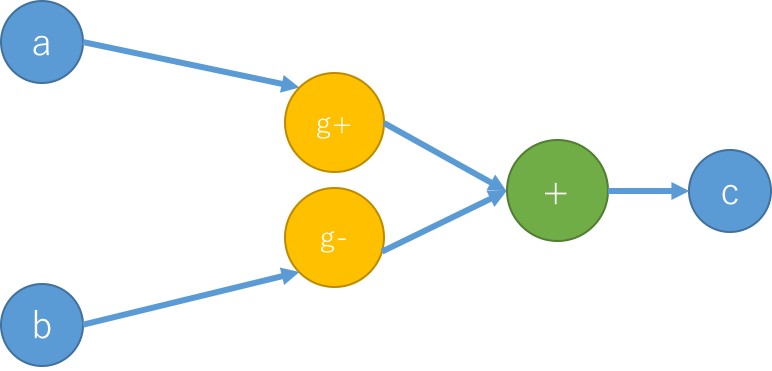
\includegraphics[height=24mm]{paper_res/conn.png}
\caption{A Net with Nonlinear Connections}
\label{fig:neurons}
\end{figure}

As synapses have two kinds: excitatory and inhibitory ones
\cite{uchizono1965characteristics,wilson1972excitatory},
we propose two categories of connections the same way.
For excitatory connections, as $\mathcal{C}_{a\rightarrow c}$
shown in figure (\ref{fig:neurons}), their signal
transferring functions are described as equation
(\ref{eq:excitatory-transfer}), in which, $\alpha\in(0,1)$
is guaranteed.
For excitatory connections,
\begin{equation}
    g^{+}(x)=\min\left(\max\left(0,\frac{x-\alpha}{1-\alpha}\right),1\right)
    \label{eq:excitatory-transfer}
\end{equation}

For inhibitory connections,
\begin{equation}
    g^{-}(x)=-g^{+}(x)
    \label{eq:inhibitory-transfer}
\end{equation}

Activation function can be any other type that constrains the output between
0 and 1, although we set activation function as the same in equation
(\ref{eq:excitatory-transfer}) as in our model.

\begin{equation}
    \sigma(x)=g^{+}(x)
    \label{eq:activation}
\end{equation}

The $\alpha$ is the only parameter, and it could be varied for
different neurons, with the same bounds of that in signal
transferring equations. The activation function of a neuron may
look like figure (\ref{fig:activation}).

\begin{figure}
    \centering
    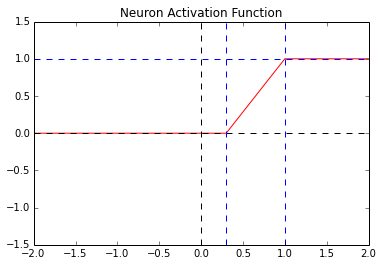
\includegraphics[height=48mm]{paper_res/activation.png}
    \caption{Activation Function of Neuron with $\alpha=0.3$}
    \label{fig:activation}
\end{figure}

For a $M$-layer neural network, The forward-computaton equation for the
$k^{\text{th}}$ neuron on $(p+1)^{\text{th}}(p=1,2,\cdots,M)$ layer,
$\mathcal{N}_{p_k}$, with the input layer denoted as the first layer, is

\begin{equation}
    o_{{p+1}_k}=\sigma(\sum_{i=1}^{N_p}g_{i\rightarrow{k}}(o_{p_i}))
    \label{eq:forward}
\end{equation}

In which, $g_{i\rightarrow{k}}$ is the signal transferring function from
$i^{\text{th}}$ neuron in $p^{\text{th}}$ layer to $k^{\text{th}}$ neuron
in $(p+1)^{\text{th}}$ layer,
and $o_{p_i}$ is the activation value of the $i^{\text{th}}$ neuron on
$p^{\text{th}}$ layer.

For network in figure (\ref{fig:neurons}), we let $o_a$, $o_b$ and $o_c$
denote the activation strengths of neuron $\mathcal{N}_a$, $\mathcal{N}_b$
and $\mathcal{N}_c$ respectively, and $\alpha_{a\rightarrow c}$,
$\alpha_{b\rightarrow c}$ as the parameters of connection
$\mathcal{C}_{a\rightarrow c}$, $\mathcal{C}_{b\rightarrow c}$ similarly.
Then we will have:

\begin{equation}
    o_c=\sigma(g^{+}(o_a)|_{\alpha=\alpha_{a\rightarrow c}} +
    g^{-}(o_b)|_{\alpha=\alpha_{b\rightarrow c}})
    \label{eq:forward-example}
\end{equation}

\subsection{Error Backpropagation For Nonlinear Connections}
While, since the equations for connections and activation function
of neurons in our model are not really differentiable, the famous
backprop algorithm cannot be applied in the training section. Thus,
we propose a training algorithm that deals with non-differentiable
situation like this.


Firstly, let's introduce two model parameters: $\xi$ and $\eta$,
they together determine the learning rate of our model. In addition,
$\xi\in(0,1)$ and $\eta\in(0,1)$. Let
$x=\sum_{i=1}^{N_p}g_{i\rightarrow{k}}(o_{p_i})$, $y=\sigma(x)$, and the given
feedback error for current neuron $\mathcal{N}_{p_k}$ is $\Delta y$.
Similarly, the feedback error for $x$ is $\Delta x$. In case parameter $\alpha$
goes to 1 and fails our equations, we propose a upper-bound $\alpha_{\max}$, which
is very close to 1 but less than 1.
Thus, the parameter updatng rules are,

\begin{equation}
    \Delta{x} = \eta\left((1-\alpha)(y+\Delta{y})+\alpha-x\right)
    \label{eq:delta-x}
\end{equation}

\begin{equation}
    \hat{\alpha}=\frac{x-y-\Delta{y}}{1-y-\Delta{y}}
    \label{eq:expected-alpha}
\end{equation}

\begin{equation}
\Delta{\alpha} =\xi\cdot\left\{
    \begin{aligned}
        &\left(\max\left(0,\hat{\alpha}\right)-\alpha\right),&\Delta{y}>0\\
        &\left(\min\left(\alpha_{\max}, \hat{\alpha}\right)-\alpha\right),&\Delta{y}<0\\
    \end{aligned}
    \right.
\label{eq:delta-alpha}
\end{equation}

Let $\Delta x_{p+1_{i\rightarrow{k}}}$ be the correction for connection
from neuron $\mathcal{N}_{p_i}$ to $\mathcal{N}_{p+1_k}$,
according to the definition of $\Delta x$ in equation (\ref{eq:delta-x}),

\begin{multline}
    \Delta x_{p+1_k} = \eta((1-\alpha_{p+1_k})(o_{p+1_k}+\Delta o_{p+1_k})\\
        +\alpha_{p+1_k}-x_{p+1_k})
    \label{eq:delta-x-real}
\end{multline}
and,
\begin{equation}
    \Delta x_{p+1_k} = \sum_{i=1}^{N_p}\Delta x_{p+1_{i\rightarrow{k}}}
    \label{eq:delta-sum}
\end{equation}

We assume that the correction strength for each connection is only related
to the activation value of the neuron which emits the connection. Thus we
will get,

\begin{equation}
    \Delta x_{p+1_{i\rightarrow{k}}} = \frac{o_{p_i}}{\sum_{j=1}^{N_p}o_{p_j}}\cdot\Delta x_{p+1_k}
    \label{eq:conn-error}
\end{equation}

Let $\alpha_{p_{i\rightarrow{k}}}$ be the parameter of the connection from the
$i^{\text{th}}$ neuron in $p^{\text{th}}$ layer to the $k^{\text{th}}$ neuron in $(p+1)^{\text{th}}$ layer.
Using equation (\ref{eq:delta-alpha}), we can update the parameters of connections.
For excitatory connections,

\begin{equation}
    \hat{\alpha}_{p_{i\rightarrow{k}}}=
        \frac{ o_{p_i}-g^{+}_{p_{i\rightarrow{k}}}(o_{p_i})-\Delta x_{p+1_{i\rightarrow{k}}} }{
        1-g^{+}_{p_{i\rightarrow{k}}}(o_{p_i})-\Delta x_{p+1_{i\rightarrow{k}}} }
    \label{eq:alpha-plus-pos}
\end{equation}

\begin{equation}
    \Delta\alpha_{p_{i\rightarrow{k}}} =\xi\cdot
    \left\{
        \begin{aligned}
            &\max\left(0,\hat{\alpha}_{p_{i\rightarrow{k}}}\right)-\alpha_{p_{i\rightarrow{k}}},\\
            &\quad\quad\Delta x_{p+1_{i\rightarrow{k}}}>0\\
            &\min\left(\alpha_{\max},\hat{\alpha}_{p_{i\rightarrow{k}}}\right)-\alpha_{p_{i\rightarrow{k}}},\\
            &\quad\quad\Delta x_{p+1_{i\rightarrow{k}}}<0\\
        \end{aligned}
        \right.
    \label{eq:conn-update-pos}
\end{equation}

For inhibitory connections, we only need to replace
$\Delta x_{p+1_{i\rightarrow{k}}}$ with $-\Delta x_{p+1_{i\rightarrow{k}}}$,
and replace $g^{+}_{p_{i\rightarrow{k}}}(o_{p_i})$ with
$-g^{-}_{p_{i\rightarrow{k}}}(o_{p_i})$ in equation (\ref{eq:alpha-plus-pos})
and (\ref{eq:conn-update-pos}),

\begin{equation}
    \hat{\alpha}_{p_{i\rightarrow{k}}}=
        \frac{ o_{p_i}+g^{-}_{p_{i\rightarrow{k}}}(o_{p_i})+\Delta x_{p+1_{i\rightarrow{k}}} }{
        1+g^{-}_{p_{i\rightarrow{k}}}(o_{p_i})+\Delta x_{p+1_{i\rightarrow{k}}} }
    \label{eq:alpha-plus-neg}
\end{equation}

\begin{equation}
    \Delta\alpha_{p_{i\rightarrow{k}}} =\xi\cdot
    \left\{
        \begin{aligned}
            &\min\left(\alpha_{\max},\hat{\alpha}_{p_{i\rightarrow{k}}}\right)-\alpha_{p_{i\rightarrow{k}}},\\
            &\quad\quad\Delta x_{p+1_{i\rightarrow{k}}}>0\\
            &\max\left(0,\hat{\alpha}_{p_{i\rightarrow{k}}}\right)-\alpha_{p_{i\rightarrow{k}}},\\
            &\quad\quad\Delta x_{p+1_{i\rightarrow{k}}}<0\\
        \end{aligned}
        \right.
    \label{eq:conn-update-neg}
\end{equation}

Biologically, A synapse can switch from excitatory to
inhibitory\cite{ganguly2001gaba}. In our model, we propose
a training strategy which allows connections switch between
excitatory and inhibitory during training process.

We propose a valve $\tau\in(0,\alpha_{\max})$, which is very close to 0 but greater
than 0, if $g_{p_{i\rightarrow{k}}}=g^{+}$, $\Delta x_{p+1_{i\rightarrow{k}}}<0$
and $\alpha_{p_{i\rightarrow{k}}}+\Delta\alpha_{p_{i\rightarrow{k}}}-\alpha_{\max}<\tau$,
then for connection $\mathcal{C}_{p_{i\rightarrow{k}}}$, let $g_{p_{i\rightarrow{k}}}=g^{-}$, this update will
switch connections from excitatory to inhibitory.
Similarly, if $g_{p_{i\rightarrow{k}}}=g^{-}$, $\Delta x_{p+1_{i\rightarrow{k}}}>0$
and $\alpha_{p_{i\rightarrow{k}}}+\Delta\alpha_{p_{i\rightarrow{k}}}-\alpha_{\max}<\tau$,
then for connection $\mathcal{C}_{p_{i\rightarrow{k}}}$, let $g_{p_{i\rightarrow{k}}}=g^{+}$, this update will
switch connections from inhibitory to excitatory.



So far we've derivated the equations for updating parameters of neurons
in $(p+1)^{\text{th}}$ layer and the parameters of connections from $p^{\text{th}}$ layer to
$(p+1)^{\text{th}}$ layer. With equation (\ref{eq:delta-x-real}),(\ref{eq:conn-error})
and (\ref{eq:delta-x}), we calculate the error of the output in the $p^{\text{th}}$ layer.
Let $\Delta o_{p_{i\rightarrow{k}}}$ be the correction for $\mathcal{N}_{p_i}$
contributed by connection $\mathcal{C}_{p_{i\rightarrow{k}}}$,
for excitatory connections,

\begin{multline}
    \Delta o^{+}_{p_{i\rightarrow{k}}} =
        \eta((1-\alpha_{p_{i\rightarrow{k}}})
        (g^{+}_{p_{i\rightarrow{k}}}(o_{p_i})+\Delta x_{p+1_{i\rightarrow{k}}})\\
        +\alpha_{p_{i\rightarrow{k}}}-o_{p_{i\rightarrow{k}}})
    \label{eq:backprop-conn-pos}
\end{multline}

For inhibitory connections,

\begin{equation}
    \Delta o^{-}_{p_{i\rightarrow{k}}} = -\Delta o^{+}_{p_{i\rightarrow{k}}}
    \label{eq:backprop-conn-neg}
\end{equation}

Then the totol correction for the output of neuron $\mathcal{N}_{p_i}$ is,

\begin{equation}
    \Delta o_{p_i} = \sum_{k=1}^{N_{p+1}}\Delta o_{p_{i\rightarrow{k}}}
    \label{eq:backprop-neuron}
\end{equation}



\section{Lateral Inhibition Nets}
\subsection{The Theory of Lateral Inhibition}
Biologically, the excitation process of neurons are inhibited by nearby excited
neurons, so called \emph{Lateral Inhibition}
\cite{amari1977dynamics,blakemore1972lateral,blakemore1970lateral}.
Researches proved that the lateral inhibition play a big role in forming patterns
in neural dynamics\cite{amari1977dynamics}.
We propose an similar mechanism in artificial neural networks, and expect to
achieve better presentation of feature map.

Let $\dot{\Upsilon}$ be the set of all nearby neurons, i.e., the neighbors of a
neuron $\mathcal{N}_0$, and $\Upsilon = \dot{\Upsilon} \cup \{\mathcal{N}_0\}$.
For general argument, if the neuron $\mathcal{N}_0$ is at position $(x,y)$
in the $i^{\text{th}}$ feature map of $p^{\text{th}}$ layer in a convolutional
neural network. Let $r\in\mathbf{N}^{+}$ be the radius of neighborhood, the center
point is $(x_0,y_0)$, thus region defined by $(x_0,y_0)\odot{r}$ is the neighborhood, and every neuron
that is away from $\mathcal{N}_0$ by an Manhattan distance within $r$ is counted in $\Upsilon$.
that is, $\Upsilon=\{\mathcal{N}_{(x,y)}\mid|x-x_0|+|y-y_0|\le r\}$, then the
lateral inhibition phase is described with equation (\ref{eq:lateral-inhibition}).

\begin{equation}
    o'_{\mathcal{N}_0}=\frac{o_{\mathcal{N}_0}}{\max(1, \sum_{\mathcal{N}_i\in\Upsilon}o_{\mathcal{N}_i})}
    \label{eq:lateral-inhibition}
\end{equation}

In equation (\ref{eq:lateral-inhibition}), $o_{\mathcal{N}_0}$ is the activation
value of neuron $\mathcal{N}_0$, and $o'_{\mathcal{N}_0}$ is the real activation
value after the lateral inhibition phase.
As the forward computing flow is changed with this additional phase, the error
backprop equations need to be updated, as in equation (\ref{eq:lateral-inhibition-backprop}).

\begin{multline}
    \Delta{o_{\mathcal{N}_0}} = ({o'}_{\mathcal{N}_0}+\Delta{o'}_{\mathcal{N}_0})\cdot
        \max(1, \sum_{\mathcal{N}_i\in\Upsilon}o_{\mathcal{N}_i} + \Delta{o'}_{\mathcal{N}_0})\\
    -{o'}_{\mathcal{N}_0}\cdot\max(1,\sum_{\mathcal{N}_i\in\Upsilon}o_{\mathcal{N}_i})
    \label{eq:lateral-inhibition-backprop}
\end{multline}

\subsection{A Visualized Instance of Lateral Inhibition}
To visualize how lateral inhibition can improve the presentation of feature maps
from original images, we propose a simple filter which only extracts perceived
luminance distribution of an image, denoted as $\mathcal{F}(\cdot)=(0.299,0.587,0.114)\cdot(r,g,b)$.
Such a filter has a size of receptive field as $1\times1$. We conduct this experiment
under \emph{Jupyter Notebook} (thanks to all supporters of this amazing staff), and
the image to test (see Fig-\ref{fig:lateral-inhibition-test-original})
is randomly chosen from Web (no offence to the president of the U.S.).

\begin{figure*}[!t]
\centering
\subfloat[The Original]{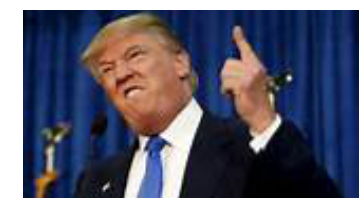
\includegraphics[width=1.5in]{paper_res/trump.png}
\label{fig:lateral-inhibition-test-original}}
\hfil
\subfloat[Luminance Filter]{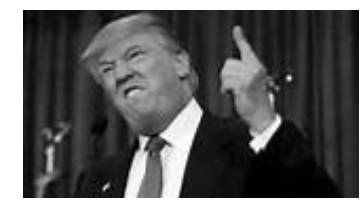
\includegraphics[width=1.5in]{paper_res/trump-filtered.png}
\label{fig:lateral-inhibition-test-filtered}}
\hfil
\subfloat[Lateral Inhibition]{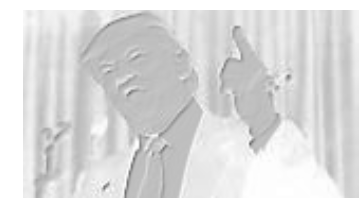
\includegraphics[width=1.5in]{paper_res/trump-lateral-inhibition.png}
\label{fig:lateral-inhibition-test-lateral-inhibition}}
\hfil
\subfloat[Binarization]{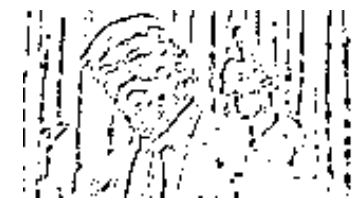
\includegraphics[width=1.5in]{paper_res/trump-binarization.png}
\label{fig:lateral-inhibition-test-binarization}}
\caption{Lateral Inhibition Visualization}
\label{fig:lateral-inhibition-test}
\end{figure*}

Using the Luminance Filter $\mathcal{F}$, we get Fig-\ref{fig:lateral-inhibition-test-filtered},
which is generally considered as a grayscale image from the original.
In conventional neural nets, such a feature map generated by this filter is
connected directly to a sub-sampling or fully-connected layer, the connection volume
and computation cost thereby are considerable, and often lead to overfitting\cite{goodfellow2013maxout}.
To overcome this, we append lateral inhibition phase immediately to each of convolution layer
before the computation process enters into next layer, expecting to make a relatively more sparse net.
The result for current case is shown as Fig-\ref{fig:lateral-inhibition-test-lateral-inhibition}.
The darker part of image is what is expected to extract. As we see, the lateral inhibition
phase performs similarly to a differential calculus of images, but with more global features
(such as luminance) remained. Let's see how this works, suppose a part of single channel image
is denoted as a float matrix $\mathbf{M}$,

\begin{equation}
\mathbf{M} = \left\{
\begin{aligned}
    0.1\quad0.0\quad0.1\quad0.9\quad0.9\quad0.9\\
    0.0\quad\mathbf{0.4}\quad0.0\quad0.9\quad\mathbf{0.9}\quad0.9\\
    0.1\quad0.0\quad0.1\quad0.9\quad0.9\quad0.9\\
\end{aligned}
\right\}
\notag
\end{equation}

Notice that only the emphasized part of matrix $\mathbf{M}$ is under observation.
Let the lateral inhibition phase be $\Omega(r)$ in which $r$ is the only parameter
for the definition of neighborhood $\Upsilon$, according to equation (\ref{eq:lateral-inhibition}),

\begin{multline}
\mathbf{M'}=\mathbf{M}\otimes\Omega(r=1) = \\
\left\{
\begin{aligned}
    0.1\quad    0.0\quad            0.1\quad    0.32\quad    0.25\quad          0.33\\
    0.0\quad    \mathbf{0.4}\quad   0.0\quad    0.25\quad    \mathbf{0.2}\quad  0.33\\
    0.1\quad    0.0\quad            0.1\quad    0.32\quad    0.25\quad          0.33\\
\end{aligned}
\right\}
\notag
\end{multline}

Before lateral inhibition phase, the left half of $\mathbf{M}$ is a 'darker' place
(the smaller, the darker),
compared to its right one. While, after $\Omega(r=1)$ is applied, the left half
remained unchanged, and the right half of $\mathbf{M'}$ is obviously suppressed,
and the right observed identity becomes surprisingly far smaller than the left.
While, we can see that the left half of the matrix still remained 'darker' than the right half,
which means lateral inhibition can keep the global features from images, and
highlights local features at the same time.

\section{Binarization of Feature Map}
\subsection{Feature Map Visualization}
Although the feature map drawn by the luminance filter is clearly visualized and understood
in last section, filters can be arbitrary and ambiguous in neural networks like CNNs,
and it thereby becomes difficult or even impossible to understand what kind of features those
filters really extract from the images.
However, if the lateral inhibition phase is employed,
we may obtain a better understanding and visualization of the feature maps, since we do not need
to care what the feature map really means, but just to know what differences are presented
among local regions of feature maps, as those differences are what truly determine which class
the input image is related to.

On the other hand, conventional visualization of feature maps simply
colorize those feature activation matrix into pactchs of image, and an average man may not get any useful information
to understand how convolutional networks work, or if they are working in a way as expected.
Recently a category of deconvolutional network is proposed to visualize the feature maps, and it seems
working well\cite{zeiler2014visualizing}. However, the method is literally too
complicated and requires much more computation, which we may not expect.

Therefore, we propose \emph{feature map binarization} to help visualize and diagnose each feature layer of CNNs
at literally no cost (the visualization is straightly one snapshot of the layer without any more
procedure as you will see).

For any type of layer at depth $p$, consisting of $N_p$ filter(s)
(actually, we may view a fully connected layer as a convolutional layer with only
single filter of which the receptive field is maximumized as the same size of last layer),
we get $N_p$ feature map(s).
For each feature map, $\Phi_{p_i},i=1,2,3,\cdots,N_p$, let $o_{p_{i_j}}'$ be the
$j^{\text{th}}$ element in map $\Phi_{p_i}'$, which is a state of $\Phi_{p_i}$ following lateral inhibition phase,
and $\dot{\Upsilon}_{p_{i_j}}$ be its neighborhood (the definition of neighborhood
preserves the same as that in lateral inhibition phase, while the parameter $r$ may be set alone),
we apply such procedure to binarize feature map $\Phi_{p_{i_j}}'$,

\begin{equation}
    \Xi_{p_{i_j}} = \{{o_{p_{i_k}}'}\mid{o_{p_{i_j}}'}-{o_{p_{i_k}}'}>\beta,o_{p_{i_k}}'\in\dot{\Upsilon}_{p_{i_j}} \}
    \label{eq:binarization-1}
\end{equation}

\begin{equation}
o_{p_{i_j}}'' =\left\{
\begin{aligned}
    1.0,\quad& \frac{\text{count}(\Xi_{p_{i_j}})}{\text{count}(\dot{\Upsilon}_{p_{i_j}})}\ge\theta \\
    0.0,\quad& \text{otherwise}\\
\end{aligned}
\right.
\label{eq:binarization-2}
\end{equation}

In equation (\ref{eq:binarization-1})(\ref{eq:binarization-2}), $\beta\in[0,+\infty]$ is the minimum gap
of activation proposed between any element in neighborhood $\dot{\Upsilon}_{p_{i_j}}$ and the interested one $o_{p_{i_j}}$,
and $\theta\in[0,1]$ is the lowerbound of the ratio of satisfied neighbors by the filter of minimum gap of activation.
Such that the binarization of feature maps is determined and only, on parameters $\left<r,\beta,\theta\right>$.

According to equation (\ref{eq:binarization-1}) and (\ref{eq:binarization-2}), we append our binarization phase
into the whole computing flow following the lateral inhibition phase. Thus we get
Fig-\ref{fig:lateral-inhibition-test-binarization}
as the binarization result of the feature map, for which we take
$\left<r,\beta,\theta\right>=\left<5,0.0,0.85\right>$.
From Fig-\ref{fig:lateral-inhibition-test-binarization},
we can clearly see what the luminance filter really extracts
from the original image, and basically how well it behaves.

\subsection{Input Determined Sparsity}
In fact, we may present the computing flow for each filter as the transformations of its feature map,
$$\mathbf{X}\longmapsto\cdots\longmapsto\Phi_{p_i}
\overset{\Omega(r)}{\longmapsto}\Phi_{p_i}'
\overset{\Psi(r,\beta,\theta)}{\longmapsto}\Phi_{p_i}''$$
in which, let $\Psi$ be the binarization phase.
We take $\Phi_{p_i}'$ as the final state of feature map generated by
filter $\mathcal{F}_{p_i}$, and $\Phi_{p_i}''$ is the mask of its sparsity.
Obviously, $\Phi_{p_i}''$ is determined by its input $\mathbf{X}$, which may be an original image.
For each different input of a net, the sparsity mask may vary,
and this is different from the Dropout\cite{hinton2012improving}
and Dropconnect\cite{wan2013regularization} regularizations, which randomly
reduce nodes or connections in a training iteration to train submodels of a net,
and consequently leading to literally twice the time cost on training\cite{hinton2012improving}.

Our method to make a net sparse relies totally on input patterns, not randomly choosing a
subset of the net model. As the feature map binarization phase indicates, it highlights
the receptive fields which have stronger responses to the input patterns,
and inhibites the others. This functionality is similarly to that of
\emph{Non-maximum suppression, NMS}\cite{dalal2005histograms}, which works well
in R-CNNs and Mask R-CNNs\cite{girshick2014rich} to get best position proposals of
objects in images. While the difference is the binarization phase in our model
does not reduce those non-maximum nodes, but keeps the majority features with
far less nodes. Thus the net made sparse with binarization phase is neither a submodel
of the original net, nor a best-object-position-proposal aided model. Our model simply
aims to reduce the redundancy of connections and speed up the training process.

\begin{figure}
\centering
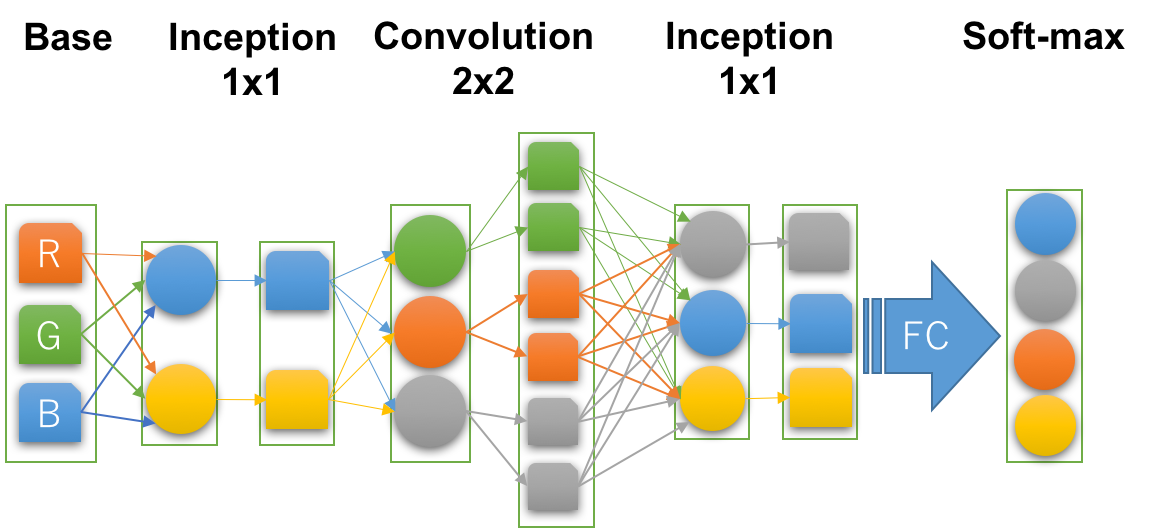
\includegraphics[width=85mm]{paper_res/arch.png}
\caption{An example of overall architectures}
\label{fig:net}
\end{figure}

For a general net of CNNs with $M$ convlayers(convolutonal layers),
we may assume that it has $N_{p}$ filters for a convlayer at depth $p$,
thus the volume of connections for this net is $O(\max(\{N_p\mid p=1,2,\cdots,M\})...)$,
With the binarization phase, we generate sparsity masks for every convlayer.
The overall architecture of our model is something like Fig-(\ref{fig:net}).


\section{Filter Polarization}
In conventional CNNs, due to huge volume of connections and sometimes insufficient training
data (big data though, not big enough yet), the redundancy of filters leads to model
overfitting and difficulty in training\cite{jaderberg2014speeding,chen2015compressing}.
Thus we propose a method called filter polarization,
it generates and pretrains those filters layer by layer, dynamically
determines the number of filters for each layer, and produces more polarized filters,
aiming to reduce the filter redundancy of nets and speed up global training.

Filter polarization algorithm contains three phase, they are executed in distinct order,
and the whole flow of three phases will iterate itself till some condition meets.

\subsection{Filter Generation}




\subsection{Filter Pretraining}



\subsection{Filter Redundancy Check}


Let $\mathcal{F}_{p_k}$ denote the $k^{\text{th}}$ filter in layer of
depth $p$, and $o_{p_k}$ be its activation value.
Firstly, we initiliazed the $p^{\text{th}}$ layer with $N_p$ filters,
for which we set the connection parameters
$\left<\alpha_{p_{k_1}},\alpha_{p_{k_2}},\cdots,\alpha_{p_{k_{N_p}}}\right>$
randomized as strictly different values.




\section{Imperical Study}
We propose a net model to achieve automatic image recognition, and it is tested
on a set of popular benchmarks.

On MNIST datasets, with no convolutional layers, we've achieved accuracy and
minimum training cost.

------------- CHART HERE -------------

On CIFAR-10 benchmark, we use convolutional layers to reduce parameter volume
and enhence model robustness. Our model performs well too.


------------ CHART HERE --------------


For small sample volume datasets like CIFAR-100 benmark, our model also outperforms
most state-of-the-art ones.


------------ CHART HERE --------------



% An example of a floating figure using the graphicx package.
% Note that \label must occur AFTER (or within) \caption.
% For figures, \caption should occur after the \includegraphics.
% Note that IEEEtran v1.7 and later has special internal code that
% is designed to preserve the operation of \label within \caption
% even when the captionsoff option is in effect. However, because
% of issues like this, it may be the safest practice to put all your
% \label just after \caption rather than within \caption{}.
%
% Reminder: the "draftcls" or "draftclsnofoot", not "draft", class
% option should be used if it is desired that the figures are to be
% displayed while in draft mode.
%
%\begin{figure}[!t]
%\centering
%\includegraphics[width=2.5in]{myfigure}
% where an .eps filename suffix will be assumed under latex,
% and a .pdf suffix will be assumed for pdflatex; or what has been declared
% via \DeclareGraphicsExtensions.
%\caption{Simulation results for the network.}
%\label{fig_sim}
%\end{figure}

% Note that the IEEE typically puts floats only at the top, even when this
% results in a large percentage of a column being occupied by floats.


% An example of a double column floating figure using two subfigures.
% (The subfig.sty package must be loaded for this to work.)
% The subfigure \label commands are set within each subfloat command,
% and the \label for the overall figure must come after \caption.
% \hfil is used as a separator to get equal spacing.
% Watch out that the combined width of all the subfigures on a
% line do not exceed the text width or a line break will occur.
%
%\begin{figure*}[!t]
%\centering
%\subfloat[Case I]{\includegraphics[width=2.5in]{box}%
%\label{fig_first_case}}
%\hfil
%\subfloat[Case II]{\includegraphics[width=2.5in]{box}%
%\label{fig_second_case}}
%\caption{Simulation results for the network.}
%\label{fig_sim}
%\end{figure*}
%
% Note that often IEEE papers with subfigures do not employ subfigure
% captions (using the optional argument to \subfloat[]), but instead will
% reference/describe all of them (a), (b), etc., within the main caption.
% Be aware that for subfig.sty to generate the (a), (b), etc., subfigure
% labels, the optional argument to \subfloat must be present. If a
% subcaption is not desired, just leave its contents blank,
% e.g., \subfloat[].


% An example of a floating table. Note that, for IEEE style tables, the
% \caption command should come BEFORE the table and, given that table
% captions serve much like titles, are usually capitalized except for words
% such as a, an, and, as, at, but, by, for, in, nor, of, on, or, the, to
% and up, which are usually not capitalized unless they are the first or
% last word of the caption. Table text will default to \footnotesize as
% the IEEE normally uses this smaller font for tables.
% The \label must come after \caption as always.
%
%\begin{table}[!t]
%% increase table row spacing, adjust to taste
%\renewcommand{\arraystretch}{1.3}
% if using array.sty, it might be a good idea to tweak the value of
% \extrarowheight as needed to properly center the text within the cells
%\caption{An Example of a Table}
%\label{table_example}
%\centering
%% Some packages, such as MDW tools, offer better commands for making tables
%% than the plain LaTeX2e tabular which is used here.
%\begin{tabular}{|c||c|}
%\hline
%One & Two\\
%\hline
%Three & Four\\
%\hline
%\end{tabular}
%\end{table}


% Note that the IEEE does not put floats in the very first column
% - or typically anywhere on the first page for that matter. Also,
% in-text middle ("here") positioning is typically not used, but it
% is allowed and encouraged for Computer Society conferences (but
% not Computer Society journals). Most IEEE journals/conferences use
% top floats exclusively.
% Note that, LaTeX2e, unlike IEEE journals/conferences, places
% footnotes above bottom floats. This can be corrected via the
% \fnbelowfloat command of the stfloats package.




\section{Conclusion}
The conclusion goes here.




% conference papers do not normally have an appendix


% use section* for acknowledgment
\section*{Acknowledgment}


The authors would like to thank...





% trigger a \newpage just before the given reference
% number - used to balance the columns on the last page
% adjust value as needed - may need to be readjusted if
% the document is modified later
%\IEEEtriggeratref{8}
% The "triggered" command can be changed if desired:
%\IEEEtriggercmd{\enlargethispage{-5in}}

% references section

% can use a bibliography generated by BibTeX as a .bbl file
% BibTeX documentation can be easily obtained at:
% http://mirror.ctan.org/biblio/bibtex/contrib/doc/
% The IEEEtran BibTeX style support page is at:
% http://www.michaelshell.org/tex/ieeetran/bibtex/
%\bibliographystyle{IEEEtran}
% argument is your BibTeX string definitions and bibliography database(s)
%\bibliography{IEEEabrv,./cites}
%
% <OR> manually copy in the resultant .bbl file
% set second argument of \begin to the number of references
% (used to reserve space for the reference number labels box)


% Generated by IEEEtran.bst, version: 1.14 (2015/08/26)
\begin{thebibliography}{10}
\providecommand{\url}[1]{#1}
\csname url@samestyle\endcsname
\providecommand{\newblock}{\relax}
\providecommand{\bibinfo}[2]{#2}
\providecommand{\BIBentrySTDinterwordspacing}{\spaceskip=0pt\relax}
\providecommand{\BIBentryALTinterwordstretchfactor}{4}
\providecommand{\BIBentryALTinterwordspacing}{\spaceskip=\fontdimen2\font plus
\BIBentryALTinterwordstretchfactor\fontdimen3\font minus
  \fontdimen4\font\relax}
\providecommand{\BIBforeignlanguage}[2]{{%
\expandafter\ifx\csname l@#1\endcsname\relax
\typeout{** WARNING: IEEEtran.bst: No hyphenation pattern has been}%
\typeout{** loaded for the language `#1'. Using the pattern for}%
\typeout{** the default language instead.}%
\else
\language=\csname l@#1\endcsname
\fi
#2}}
\providecommand{\BIBdecl}{\relax}
\BIBdecl

\bibitem{fukushima1979neural}
K.~Fukushima, ``Neural network model for a mechanism of pattern recognition
unaffected by shift in position- neocognitron,'' \emph{ELECTRON. \& COMMUN.
JAPAN}, vol.~62, no.~10, pp. 11--18, 1979.

\bibitem{weng1992cresceptron}
J.~Weng, N.~Ahuja, and T.~S. Huang, ``Cresceptron: a self-organizing neural
network which grows adaptively,'' in \emph{Neural Networks, 1992. IJCNN.,
International Joint Conference on}, vol.~1.\hskip 1em plus 0.5em minus
0.4em\relax IEEE, 1992, pp. 576--581.

\bibitem{lecun1989backpropagation}
Y.~LeCun, B.~Boser, J.~S. Denker, D.~Henderson, R.~E. Howard, W.~Hubbard, and
L.~D. Jackel, ``Backpropagation applied to handwritten zip code
recognition,'' \emph{Neural computation}, vol.~1, no.~4, pp. 541--551, 1989.

\bibitem{ciresan2011flexible}
D.~C. Ciresan, U.~Meier, J.~Masci, L.~Maria~Gambardella, and J.~Schmidhuber,
``Flexible, high performance convolutional neural networks for image
classification,'' in \emph{IJCAI Proceedings-International Joint Conference
on Artificial Intelligence}, vol.~22, no.~1.\hskip 1em plus 0.5em minus
0.4em\relax Barcelona, Spain, 2011, p. 1237.

\bibitem{ciregan2012multi}
D.~Ciregan, U.~Meier, and J.~Schmidhuber, ``Multi-column deep neural networks
for image classification,'' in \emph{Computer Vision and Pattern Recognition
(CVPR), 2012 IEEE Conference on}.\hskip 1em plus 0.5em minus 0.4em\relax
IEEE, 2012, pp. 3642--3649.

\bibitem{krizhevsky2012imagenet}
A.~Krizhevsky, I.~Sutskever, and G.~E. Hinton, ``Imagenet classification with
deep convolutional neural networks,'' in \emph{Advances in neural information
processing systems}, 2012, pp. 1097--1105.

\bibitem{goodfellow2013maxout}
I.~J. Goodfellow, D.~Warde-Farley, M.~Mirza, A.~C. Courville, and Y.~Bengio,
``Maxout networks.'' \emph{ICML (3)}, vol.~28, pp. 1319--1327, 2013.

\bibitem{lin2013network}
M.~Lin, Q.~Chen, and S.~Yan, ``Network in network,'' \emph{arXiv preprint
arXiv:1312.4400}, 2013.

\bibitem{cirecsan2013mitosis}
D.~C. Cire{\c{s}}an, A.~Giusti, L.~M. Gambardella, and J.~Schmidhuber,
``Mitosis detection in breast cancer histology images with deep neural
networks,'' in \emph{International Conference on Medical Image Computing and
Computer-assisted Intervention}.\hskip 1em plus 0.5em minus 0.4em\relax
Springer, 2013, pp. 411--418.

\bibitem{ciresan2012deep}
D.~Ciresan, A.~Giusti, L.~M. Gambardella, and J.~Schmidhuber, ``Deep neural
networks segment neuronal membranes in electron microscopy images,'' in
\emph{Advances in neural information processing systems}, 2012, pp.
2843--2851.

\bibitem{farabet2013learning}
C.~Farabet, C.~Couprie, L.~Najman, and Y.~LeCun, ``Learning hierarchical
features for scene labeling,'' \emph{IEEE transactions on pattern analysis
and machine intelligence}, vol.~35, no.~8, pp. 1915--1929, 2013.

\bibitem{sermanet2013pedestrian}
P.~Sermanet, K.~Kavukcuoglu, S.~Chintala, and Y.~LeCun, ``Pedestrian detection
with unsupervised multi-stage feature learning,'' in \emph{Proceedings of the
IEEE Conference on Computer Vision and Pattern Recognition}, 2013, pp.
3626--3633.

\bibitem{schmidhuber2015deep}
J.~Schmidhuber, ``Deep learning in neural networks: An overview,'' \emph{Neural
networks}, vol.~61, pp. 85--117, 2015.

\bibitem{gabor1946theory}
D.~Gabor, ``Theory of communication. part 1: The analysis of information,''
\emph{Journal of the Institution of Electrical Engineers-Part III: Radio and
Communication Engineering}, vol.~93, no.~26, pp. 429--441, 1946.

\bibitem{zeiler2014visualizing}
M.~D. Zeiler and R.~Fergus, ``Visualizing and understanding convolutional
networks,'' in \emph{European conference on computer vision}.\hskip 1em plus
0.5em minus 0.4em\relax Springer, 2014, pp. 818--833.

\bibitem{hall1905textbook}
W.~S. Hall, \emph{A Textbook of physiology}.\hskip 1em plus 0.5em minus
0.4em\relax Lea, 1905.

\bibitem{bayliss1908reciprocal}
W.~Bayliss, ``On reciprocal innervation in vaso-motor reflexes and the action
of strychnine and of chloroform thereon,'' \emph{Proceedings of the Royal
Society of London. Series B, Containing Papers of a Biological Character},
vol.~80, no. 541, pp. 339--375, 1908.

\bibitem{gerard1941interaction}
R.~Gerard, ``The interaction of neurones,'' \emph{Ohio J. Sci}, vol.~41, pp.
160--172, 1941.

\bibitem{jain1996artificial}
A.~K. Jain, J.~Mao, and K.~M. Mohiuddin, ``Artificial neural networks: A
tutorial,'' \emph{Computer}, vol.~29, no.~3, pp. 31--44, 1996.

\bibitem{nair2010rectified}
V.~Nair and G.~E. Hinton, ``Rectified linear units improve restricted boltzmann
machines,'' in \emph{Proceedings of the 27th international conference on
machine learning (ICML-10)}, 2010, pp. 807--814.

\bibitem{gray1959axo}
E.~G. Gray, ``Axo-somatic and axo-dendritic synapses of the cerebral cortex: an
electron microscope study,'' \emph{Journal of anatomy}, vol.~93, no. Pt 4, p.
420, 1959.

\bibitem{harvey2007locally}
C.~D. Harvey and K.~Svoboda, ``Locally dynamic synaptic learning rules in
pyramidal neuron dendrites,'' \emph{Nature}, vol. 450, no. 7173, pp.
1195--1200, 2007.

\bibitem{uchizono1965characteristics}
K.~Uchizono, ``Characteristics of excitatory and inhibitory synapses in the
central nervous system of the cat,'' \emph{Nature}, vol. 207, no. 4997, pp.
642--643, 1965.

\bibitem{wilson1972excitatory}
H.~R. Wilson and J.~D. Cowan, ``Excitatory and inhibitory interactions in
localized populations of model neurons,'' \emph{Biophysical journal},
vol.~12, no.~1, pp. 1--24, 1972.

\bibitem{ganguly2001gaba}
K.~Ganguly, A.~F. Schinder, S.~T. Wong, and M.-m. Poo, ``Gaba itself promotes
the developmental switch of neuronal gabaergic responses from excitation to
inhibition,'' \emph{Cell}, vol. 105, no.~4, pp. 521--532, 2001.

\bibitem{amari1977dynamics}
S.-i. Amari, ``Dynamics of pattern formation in lateral-inhibition type neural
  fields,'' \emph{Biological cybernetics}, vol.~27, no.~2, pp. 77--87, 1977.

\bibitem{blakemore1972lateral}
C.~Blakemore and E.~A. Tobin, ``Lateral inhibition between orientation
detectors in the cat's visual cortex,'' \emph{Experimental Brain Research},
vol.~15, no.~4, pp. 439--440, 1972.

\bibitem{blakemore1970lateral}
C.~Blakemore, R.~H. Carpenter, and M.~A. Georgeson, ``Lateral inhibition
between orientation detectors in the human visual system.'' \emph{Nature},
1970.

\bibitem{jaderberg2014speeding}
M.~Jaderberg, A.~Vedaldi, and A.~Zisserman, ``Speeding up convolutional neural
networks with low rank expansions,'' \emph{arXiv preprint arXiv:1405.3866},
2014.

\bibitem{chen2015compressing}
W.~Chen, J.~T. Wilson, S.~Tyree, K.~Q. Weinberger, and Y.~Chen, ``Compressing
convolutional neural networks,'' \emph{arXiv preprint arXiv:1506.04449},
2015.

\bibitem{masci2011stacked}
J.~Masci, U.~Meier, D.~Cire{\c{s}}an, and J.~Schmidhuber, ``Stacked
convolutional auto-encoders for hierarchical feature extraction,''
\emph{Artificial Neural Networks and Machine Learning--ICANN 2011}, pp.
52--59, 2011.

\bibitem{hinton2012improving}
G.~E. Hinton, N.~Srivastava, A.~Krizhevsky, I.~Sutskever, and R.~R.
Salakhutdinov, ``Improving neural networks by preventing co-adaptation of
feature detectors,'' \emph{arXiv preprint arXiv:1207.0580}, 2012.

\bibitem{wan2013regularization}
L.~Wan, M.~Zeiler, S.~Zhang, Y.~L. Cun, and R.~Fergus, ``Regularization of
neural networks using dropconnect,'' in \emph{Proceedings of the 30th
International Conference on Machine Learning (ICML-13)}, 2013, pp.
1058--1066.

\bibitem{dalal2005histograms}
N.~Dalal and B.~Triggs, ``Histograms of oriented gradients for human
detection,'' in \emph{Computer Vision and Pattern Recognition, 2005. CVPR
2005. IEEE Computer Society Conference on}, vol.~1.\hskip 1em plus 0.5em
minus 0.4em\relax IEEE, 2005, pp. 886--893.

\bibitem{girshick2014rich}
R.~Girshick, J.~Donahue, T.~Darrell, and J.~Malik, ``Rich feature hierarchies
for accurate object detection and semantic segmentation,'' in
\emph{Proceedings of the IEEE conference on computer vision and pattern
recognition}, 2014, pp. 580--587.

\end{thebibliography}



% that's all folks
\end{document}
